%%%%%%%%%%%%%%%%%%%%%%%%%%%%%%%%%%%%%%%%%
% Journal Article
% LaTeX Template
% Version 1.3 (9/9/13)
%
% This template has been downloaded from:
% http://www.LaTeXTemplates.com
%
% Original author:
% Frits Wenneker (http://www.howtotex.com)
%
% License:
% CC BY-NC-SA 3.0 (http://creativecommons.org/licenses/by-nc-sa/3.0/)
%
%%%%%%%%%%%%%%%%%%%%%%%%%%%%%%%%%%%%%%%%%

%----------------------------------------------------------------------------------------
%	PACKAGES AND OTHER DOCUMENT CONFIGURATIONS
%----------------------------------------------------------------------------------------

\documentclass[hidelinks]{article}

\usepackage{lipsum} % Package to generate dummy text throughout this template
\usepackage{ amssymb }
\usepackage{ amsmath }
\usepackage{graphicx}
\usepackage[english]{babel}

\usepackage[sc]{mathpazo} % Use the Palatino font
\usepackage[T1]{fontenc} % Use 8-bit encoding that has 256 glyphs
\linespread{1.05} % Line spacing - Palatino needs more space between lines
\usepackage{microtype} % Slightly tweak font spacing for aesthetics

\usepackage[hmarginratio=1:1,top=32mm,columnsep=20pt]{geometry} % Document margins
\usepackage{multicol} % Used for the two-column layout of the document
\usepackage[hang, small,labelfont=bf,up,textfont=it,up]{caption} % Custom captions under/above floats in tables or figures
\usepackage{booktabs} % Horizontal rules in tables
\usepackage{float} % Required for tables and figures in the multi-column environment - they need to be placed in specific locations with the [H] (e.g. \begin{table}[H])
\usepackage{fancyref} % For hyperlinks in the PDF

\usepackage{lettrine} % The lettrine is the first enlarged letter at the beginning of the text
\usepackage{paralist} % Used for the compactitem environment which makes bullet points with less space between them

\usepackage{abstract} % Allows abstract customization
\renewcommand{\abstractnamefont}{\normalfont\bfseries} % Set the "Abstract" text to bold
\renewcommand{\abstracttextfont}{\normalfont\small\itshape} % Set the abstract itself to small italic text

\usepackage{titlesec} % Allows customization of titles
\renewcommand\thesection{\Roman{section}} % Roman numerals for the sections
\renewcommand\thesubsection{\Roman{subsection}} % Roman numerals for subsections
\titleformat{\section}[block]{\large\scshape\centering}{\thesection.}{1em}{} % Change the look of the section titles
\titleformat{\subsection}[block]{\large}{\thesubsection.}{1em}{} % Change the look of the section titles

\usepackage{fancyhdr} % Headers and footers
\pagestyle{fancy} % All pages have headers and footers
\fancyhead{} % Blank out the default header
\fancyfoot{} % Blank out the default footer
\fancyhead[C]{Physics 3200 $\bullet$ Jerin Roberts $\bullet$ April 2014} % Custom header text
\fancyfoot[RO,LE]{\thepage} % Custom footer text

%----------------------------------------------------------------------------------------
%	TITLE SECTION
%----------------------------------------------------------------------------------------

\title{\vspace{-15mm}\fontsize{15pt}{10pt}\selectfont\textbf{Modeling a Triatomic Molecule with Mass-Spring System}} % Article title

\author{
\large
\textsc{Jerin Roberts}\\[2mm] % Your name
\normalsize Thompson Rivers University \\ % Your institution
\normalsize {robertsj10@mytru.ca} % Your email address
\vspace{-5mm}
}
\date{}

%----------------------------------------------------------------------------------------

\begin{document}

\maketitle % Insert title

\thispagestyle{fancy} % All pages have headers and footers

%----------------------------------------------------------------------------------------
%	ABSTRACT
%----------------------------------------------------------------------------------------

\begin{abstract}

The motion of a triatomic molecule may be modeled using a simplified mass-spring system. Employing Lagrangian mechanics we will solve for the equations of motion that govern the molecule. Using matrix operations one can find complex solutions that will satisfy all the equations of motion simultaneously. By only considering the real part of the solutions the motion, including the modes and frequencies of oscillation, of the molecule will be found.

\end{abstract}

%----------------------------------------------------------------------------------------
%	ARTICLE CONTENTS
%----------------------------------------------------------------------------------------

\begin{multicols}{2} % Two-column layout throughout the main article text

\section{Introduction}


Atoms are the building blocks for molecules and compounds and can take on many configurations. Atoms form bonds to lower the energy of an atomic system. The bonds are generally a representation of electronic orbital interactions and as a result can take on several different configurations. In ionic bonds electrons are transferred between two atoms which results in a mutual electrostatic attraction which keeps the atoms together. 
\begin{figure}[H]
\centering
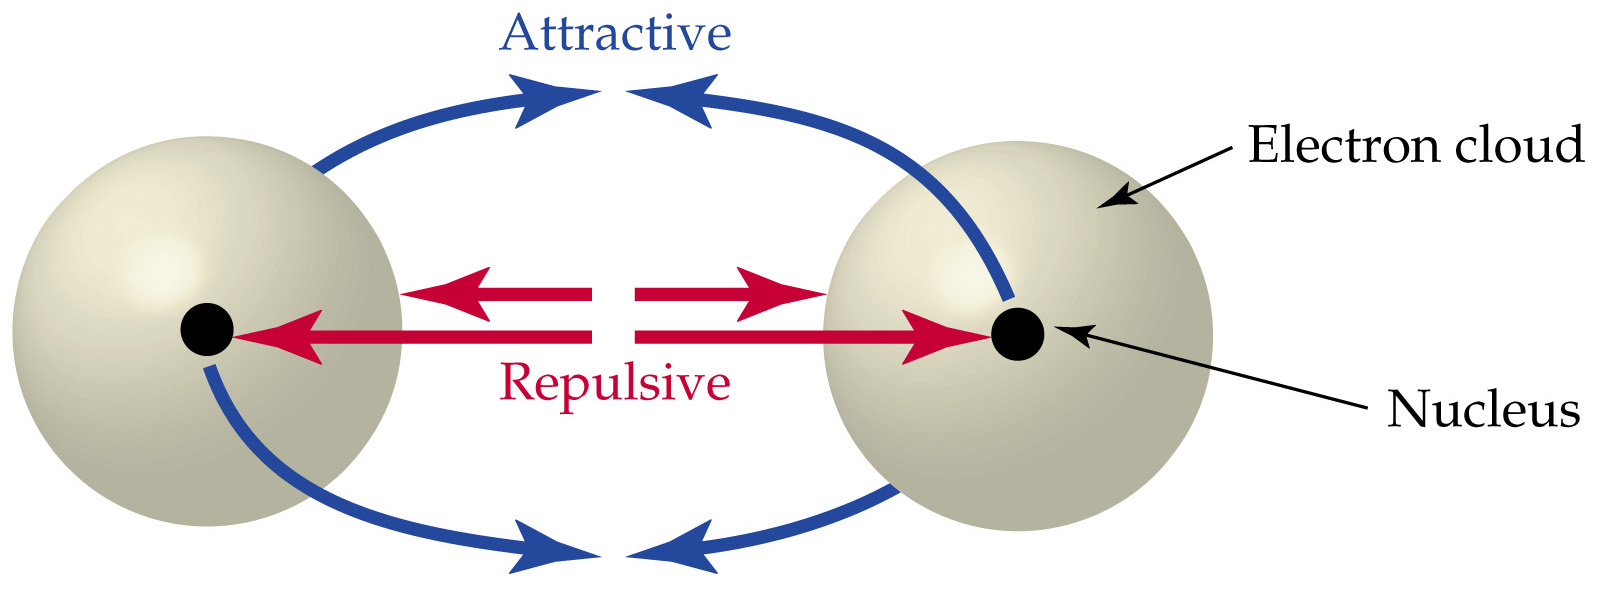
\includegraphics[width=\linewidth]{cloud}
\caption{The electrostatic intereations found in chemical bonds.\cite{2}}
\label{fig1}
\end{figure}
Covalent bonds are generated between two atoms when both required an electron to satisfy the outer valence shell, as result the energy of the system is lowered when an electron is shared. When a bond is formed each atom is trapped in a potential dip generated by its partner. Generally these wells form as a product of repulsive and attractive electrostatic forces (Figure \ref{fig1}). The positive nucleus of each atom is attracted to the others electron cloud but repelled by their nucleus and therefore the atoms are trapped or bounded. The equilibrium of these two interactions corresponds to the point of lowest energy.
\begin{figure}[H]
\centering
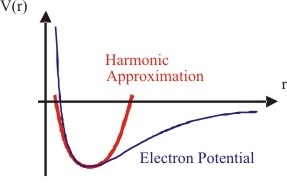
\includegraphics[width=\linewidth]{harm}
\caption{The electronic potential well and the approximation of a harmonic system.\cite{3}}
\label{fig2}
\end{figure}
If one imagines a gravitational potential as a parabolic curve and a particle that can slide on the surface of that curve, the particle will always want to slide to the lowest point. If no additional energy is added initially the particle will sit at the apex of the parabola. If one gives the particle a push, or more specifically greater energy, the particle will slide up one side, and as doing so it loses energy and eventually slides back down. Ignoring drag and friction the particle will continue to overshoot the lowest energy state, and therefore will oscillate about the equilibrium point. This is known as simple harmonic motion \cite{1}. The potential that describes an atom while bonded can closely be modeled by a potential function of a harmonic oscillator as shown in Figure \ref{fig2}. A simple harmonic oscillator that has been extensively studied and analysed is the mass-spring system. Therefore many atomic models can be analysed and solved with simple mass-spring systems.

%*******************************************************************************************

\section{Lagrangian Mechanics}

If one wishes to know the possible motions of a system it is best to attain and solve its equations of motion. These can be derived from newton's laws of motion, however this is an arduous task as Newtonian mechanics would require solving for the time-varying constraint forces of the mass spring-system. Lagrangian mechanics offers an easier method for solving the mass-spring problem. Lagrangian mechanics is based on the principle of least action and can be applied to all conserved or non-conserved systems. \cite{1}

\begin{equation}
\label{Leed}
\mathcal{L}=T-U
\end{equation}
\begin{equation}
\label{ELeed}
\frac{\partial \mathcal{L}}{\partial q}=\frac{d}{dt}\frac{\partial \mathcal{L}}{\partial \dot{q}}
\end{equation}

Solving the Lagrange equations is equivalent to finding the path for which the integral of the Lagrangian over time is constant. The main component of Lagrangian mechanics is the Lagrangian function, which describes the dynamics of the entire system in terms of kinetic and potential energies (eq.\ref{Leed}). With the Lagrangian and the Euler-Lagrange equation, the equations of motion for the system can be easily found. The Euler-Lagrange equation can be used to solve any system with n-degrees of freedom where each degree of freedom will represent a generalized coordinate (eq.\ref{ELeed}). For each generalized coordinate an equation of motion will be generated \cite{1}. 

%***********************************************************************************************

\section{Triatomic Model}



For our problem we are considering the possible motions of a linear triatomic molecule (Figure \ref{model}). A central mass labelled M is connected on either side to masses m by springs both with a spring constant k. In this model the masses are only allowed only to move in the horizontal x direction. The displacement of each mass is measure from the rest or relaxed state of the system or more specifically the point in which the spring contains no stored energy. Our system contains three degrees of freedom which correspond to the chosen generalized coordinates of $x_1$ $x_2$, and $x_3$. All coordinates are measured from the relaxed positions of the masses $m_1$, $m_2$, $m_3$ which are of mass m, M, and m respectively. 

\begin{figure}[H]
\centering
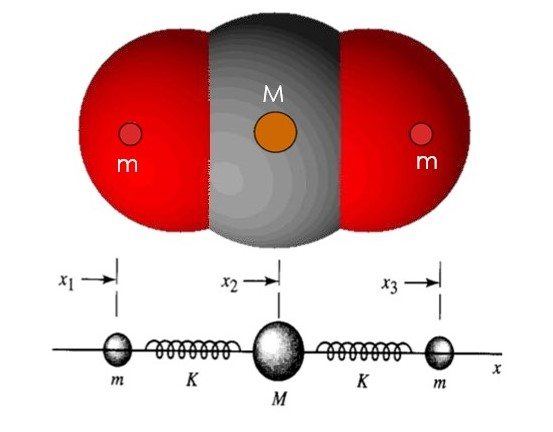
\includegraphics[width=\linewidth]{model}
\caption{the generalized coordinates of our system.}
\label{model}
\end{figure}



The total kinetic energy of the system is just the sum of all the kinetic energies for each of the masses which is displayed as equation \ref{kinetic}. Since our model negates external forces, the potential of the system is solely due to the extension or compression of the springs. Therefore the potential energy of the system is the sum of the potential produced by each spring display by equation \ref{potential}.

\begin{equation}
\label{kinetic}
T= \frac{1}{2}m(\dot{x}_1)^2+\frac{1}{2}M(\dot{x_2})^2+\frac{1}{2}m(\dot{x_3})^2
\end{equation}

\begin{equation}
U=\frac{1}{2}k(x_2-x_1)^2+\frac{1}{2}k(x_3-x_2)^2
\label{potential}
\end{equation}

The Lagrangian is then found to be the difference between the sums of the kinetic and potential energies from equation \ref{Leed}. To find the equations of motion for each generalized coordinate we apply the Euler-Lagrange equation to each coordinate (Equation \ref{ELO}). In our case the $\frac{\partial \mathcal{L}}{\partial x_i}$ term will give us our generalized force and the $\frac{\partial \mathcal{L}}{\partial \dot{x}_i}$ will give us the generalized momentum.
\begin{equation}
\begin{split}
\frac{\partial \mathcal{L}}{\partial x_i}=\frac{d}{dt}\frac{\partial \mathcal{L}}{\partial \dot{x}_i} \\
i = 1,2,3
\end{split}
\label{ELO}
\end{equation} 

This gives us the equations of motion for a triatomic system using generalized coordinates $x_1, x_2,$ and $ x_3$ which are equations \ref{num1}, \ref{num2}, and \ref{num3} respectively. 

\begin{equation}
\label{num1}
m\ddot{x}_1=k(x_1-x_2) 
\end{equation}

\begin{equation}
\label{num2}
m\ddot{x}_2=k(2x_2-x_1-x_3)
\end{equation}

\begin{equation}
\label{num3}
m\ddot{x}_3=k(x_3-x_2)
\end{equation}

These are coupled, 2$^{nd}$ order linear differential equations which can be solved using both numerical and mathematical processes.

%*************************************************************************************


\section{Matrix Operations}

Since the equations of motion are coupled its best to express the equations as a tensor (eq.\ref{matrixe}). These matrices satisfy the matrix expression displayed as equation \ref{matrix} where $\mathbf{M}$ is the mass matrix and $\mathbf{K}$ is the spring constant matrix. If we can find a solution that satisfies the matrix expression then effectively we have found a solution that is able to simultaneously satisfy all the equations of motion.

\begin{equation}
\label{matrixe}
\begin{split}
\begin{bmatrix}
m & 0 & 0 \\
0 & M & 0 \\
0 & 0 & m 
\end{bmatrix}
\begin{bmatrix}
\ddot{x}_1 \\
\ddot{x}_2 \\
\ddot{x}_3
\end{bmatrix}
=\\
\begin{bmatrix}
k & -k & 0 \\
-k & 2k & -k \\
0 & -k & k 
\end{bmatrix}
\begin{bmatrix}
x_1 \\
x_2 \\
x_3
\end{bmatrix}
\end{split}
\end{equation}

\begin{equation}
\label{matrix}
\mathbf{M\ddot{x}}=\mathbf{Kx}
\end{equation}



We expect the masses to oscillate sinusoidally with the frequency $\omega$. Therefore we find that equations \ref{cos} and \ref{sin} indeed satisfy the matrix expression.

\begin{equation}
\label{cos}
\begin{split}
x_j(t) = a_jcos(\omega t)\\
j=1,2,3...
\end{split}
\end{equation}

\begin{equation}
\label{sin}
x_j(t) = b_jsin(\omega t)
\end{equation}

These expressions can be further simplified by combining them into a set of complex solutions (\ref{exp}) \cite{1}. 

\begin{equation}
\label{exp}
x_j(t) = z_je^{i\omega t}
\end{equation}

Since we are working with matrices we can express equation \ref{exp} as a matrix solution (eq.\ref{expm}). It should be noted that when we find such solutions that the actual motion will be only described by the real part of $z(t)$ such that $x(t)=Realz(t)$ \cite{1}.
\begin{equation}
\label{expm}
z(t) = \underline{Z}e^{i\omega t}
\end{equation}

When we substitute the solution (eq.\ref{expm}) into equation \ref{matrix}, while cancelling the common exponent, we attain equation \ref{ev} which happens to be the generalized eigenvalue equation where $\omega^2$ is the eigenvalue and $\underline{Z}$ is the eigenvector.


\begin{equation}
\label{ev}
(K-\omega^2M)\underline{Z}=\underline{0}
\end{equation}

%*********************************************************************************************


\section{Solving the Eigenvalue Equation}

The eigenvalue equation can be used to find the natural frequencies and the normal modes of oscillation. Therefore finding solutions for $\omega^2$ that satisfy the eigenvalue equation is required. If the matrix in equation \ref{ev} has a non-zero determinant then the only solution that exists is $\underline{Z}=0$, which corresponds to no motion at all. However if the determinant is equal to zero (eq.\ref{det}, then their exists non-trivial solutions and therefore a solution of our assumed form to the equations of motion for the triatomic system \cite{1}.

\begin{equation}
\label{det}
det(K-\omega^2M)=0
\end{equation}

Solving the determinant yields equation \ref{quad}. This equation can be solved for three distinct roots which are displayed in equation \ref{roots}.

\begin{equation}
\label{quad}
\omega^2(k-\omega^2m)(-k(2m+M)+mM\omega^2)=0
\end{equation}

\begin{equation}
\label{roots}
\begin{split}
\omega_1=0\\
\omega_2=\sqrt{\frac{k}{m}}\\
\omega_3=\sqrt{\frac{2k}{M}+\frac{k}{m}}
\end{split}
\end{equation}

These roots represent the frequencies for the modes of oscillation. The question remains however, which of these modes are these frequencies describing? Hence the eigenvectors are needed in order to find the modes of oscillation. The modes which correspond to $z_1, z_2,$ and $z_3$ eigenvectors are solved by substituting the corresponding eigenvalues back into the eigenvalue equation and solving for $\underline{Z}$ which are given by equations \ref{zed1} to \ref{zed3}.

\begin{equation}
\label{zed1}
z_1=
\begin{bmatrix}
1\\
1\\
1
\end{bmatrix}
\end{equation}
\begin{equation}
\label{zed2}
z_2=
\begin{bmatrix}
-1\\
0\\
1
\end{bmatrix}
\end{equation}
\begin{equation}
\label{zed3}
z_3=
\begin{bmatrix}
1\\
\frac{-m}{2M}\\
1
\end{bmatrix}
\end{equation}

With the eigenvalues and eigenvectors we can sub these back into our assumed solution which will give us the solutions that simultaneously satisfy our equations of motion. The solutions are displayed as equations \ref{sol1} to \ref{sol3}.

\begin{equation}
\label{sol1}
x_1(t)=
\begin{bmatrix}
1\\
1\\
1
\end{bmatrix}
f(t)
\end{equation}
\begin{equation}
\label{sol2}
x_2(t)=
\begin{bmatrix}
-1\\
0\\
1
\end{bmatrix}
e^{i\sqrt{\frac{k}{m}t}}
\end{equation}

\begin{equation}
\label{sol3}
x_3(t)=
\begin{bmatrix}
1\\
\frac{-m}{2M}\\
1
\end{bmatrix}
e^{i\sqrt{\frac{2k}{M}+\frac{k}{m}t}}
\end{equation}

%*********************************************************************************************


\section{ Modes of Oscillation}

The eigenvectors found in the previous section gives us a lot of information about the system. It not only shows which masses are in motion for certain modes, but can also describe the relative phases of the individual motions. The eigenvalue displayed by equation \ref{zed1} shows the same magnitude of motion for all masses in the same direction with no oscillating frequency. This type of mode describes the motion of the system as being invariant under coordinate translation \cite{1}. This motion is demonstrated in figure \ref{mode1}.

\begin{figure}[H]
\centering
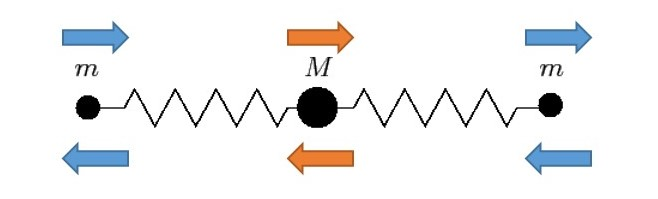
\includegraphics[width=\linewidth]{111}
\caption{Displays the type of motion associated with the $\omega_1$ mode frequency which is equal to zero, ie translational motion}
\label{mode1}
\end{figure}

The second mode of oscillation which corresponds to the $\omega_2$ frequency is displayed in figure \ref{mode2}. In this motion the outer masses m are out of phase with each other while the central mass can be treated as stationary. The outer masses move in and then out at frequency $\omega_2$. The central mass will remain stationary relative to the other two masses because the sum of the forces on it at any given time is zero, therefore its motion has no time dependence and can be treated as non-existent 

\begin{figure}[H]
\centering
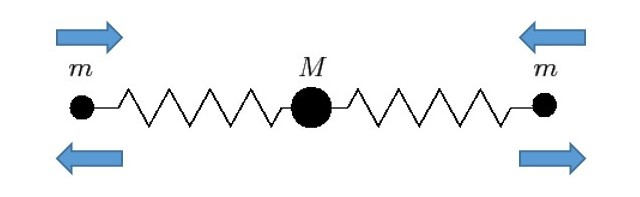
\includegraphics[width=\linewidth]{10-1}
\caption{Displays the type of motion associated with the $\omega_2$ mode frequency: The m masses are out of phase with each while mass M can be treated as stationary}
\label{mode2}
\end{figure}

The third and last mode of oscillation describes the out of phase motion between the outer and central masses moving a frequency $\omega_3$. More specifically as shown in figure \ref{mode3} while both the outer masses are moving in the +x direction the central mass is moving in the -x direction. .

\begin{figure}[H]
\centering
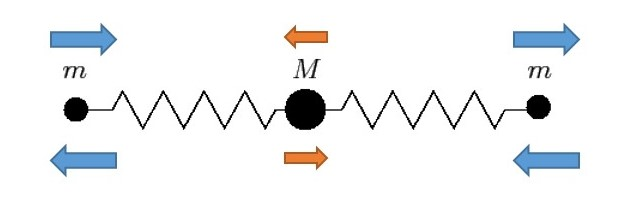
\includegraphics[width=\linewidth]{1-11}
\caption{Displays the type of motion associated with the $\omega_3$ mode frequency: The outer masses are in phase with each other and are out of phase with central mass M}
\label{mode3}
\end{figure}

It should be noted that the center of mass of the system remains constant as there are no external forces present, however the central mass M, given the outer m masses are massive enough, will oscillate about the center of mass. This is due to the fact that the sum of the forces on the central mass is non-zero. This is a directly observed feature of the eigenvector for this mode. The motion of the central mass is denoted by the ratio between the central and outer masses.

%*************************************************************************************************


\section{Limiting Cases: 2nd Mode}
In order to confirm the validity of the solutions for the equations of motion its best to look at the limiting cases for each. More specifically do the equations make physical sense when the variables are taken to minimum and maximum extremes? Looking at equation \ref{sol3} we see the solutions are completely independent of the size of the central mass M. This means the system should act similarly to a system without a central mass. Equation \ref{2mass} represents a solution for the motion of a two mass system connected by a single spring. We see that this equation closely resembles equation \ref{sol2}. Because of the presence of two springs in the triatomic model when the central mass is motionless the springs are added in series. This means the effective spring constant for the combination of the two springs is halved. Once this is accounted for we see the solution for the two mass system matches the 2nd solution for the triatomic system during out of phase motion as physically expected.

\begin{equation}
\label{2mass}
\begin{split}
x(t)=
\begin{bmatrix}
-1\\
1
\end{bmatrix}
e^{i\sqrt{\frac{2k'}{m}t}}
\\
k'=\frac{k}{2}
\end{split}
\end{equation}
Since the variables of the system are the masses and the spring constants it is a good idea to see how the solutions behave when either of these go to zero or infinity. For equation \ref{sol2} we see the frequency of the outer masses or atoms is dependent on their mass as well as the spring constants of the springs. If the spring constant were zero, we would see the exponential term disappear and as expected we see there would be no spring force to return the masses back to the relaxed position, and therefore the motion of the masses would continue indefinitely in opposite directions. This scenario would also be expected if the mass of the outer atoms went to infinity, and therefore the springs would not provide sufficient force to retard the outer atoms motion. This example is validated through solution \ref{sol2} when mass of the outer atoms gets infinitely large. It is also interesting to note that if k and m increase or decrease at the same rates then oscillations about this mode will still continue.

\section{Limiting Cases: 3rd Mode}
For solution \ref{sol3} as from the previous section when the spring constant k goes to zero we find the motion becomes continuous and non-oscillating. More specifically the springs provide no resistance to the masses and they continue to move unimpeded with their initial motion. When M or m approaches zero we see the frequency gets very large and the triatomic molecule acts extremely stiff where oscillations occurring would be too high to detect. Looking at the scenario when M becomes infinity large, we expect the motion to be exhibited only by the outer masses. Looking at equation \ref{sol3} we see that as M goes to infinity the $\frac{2k}{M}$ from the frequency and the $\frac{-m}{2M}$ term both go to zero. The new resulting equation is shown as equation \ref{M0}.

\begin{equation}
\label{M0}
x_3(t)=
\begin{bmatrix}
1\\
0\\
1
\end{bmatrix}
e^{i\sqrt{\frac{k}{m}t}}
\end{equation}
This as expected shows the central mass will have zero motion. This is due to its relatively large inertia, the smaller outer masses have little effect on moving the infinitely large central mass. The outer masses will still exhibit oscillatory motion at a frequency denoted by their mass. Conversely when the outer masses m approach infinity we would expect only the central mass to exhibit oscillatory motion. Equation \ref{MI} displays the effect when m approaches infinity.
\begin{equation}
\label{MI}
x_3(t)=
\begin{bmatrix}
1\\
-\infty \\
1
\end{bmatrix}
e^{i\sqrt{\frac{2k}{M}t}}
\end{equation}

The matrix evidently shows that all the motion will be exhibited by the central mass, moving at a frequency denoted by its own mass, as we would expect physically. The outer masses will exhibit little to no motion at all which is due to their large inertia.

\section{Summary}
In order to find solutions to the possible motions of a triatomic system we set forth to model it using a simple mass-spring system. By finding the Lagrangian and solving the Euler-Lagrange equation, we were able to solve for the equations of motion. Since the equations of motion were coupled between the three generalized coordinates it made sense to write them in matrix form and by finding a solution to the matrix expression we were able to find solutions that simultaneously satisfied all the equations of motion. We validate the solutions to the equations of motion by investigating the limiting cases and were able to conclude they adequately describe a very simplified triatomic molecule.

 
 
 



%----------------------------------------------------------------------------------------
%	REFERENCE LIST
%----------------------------------------------------------------------------------------

\begin{thebibliography}{99} % Bibliography - this is intentionally simple in this template

\bibitem[1]{1}
Taylor, R.~J. (2005).
\newblock Classical Mechanics
\newblock {\em University Science Books}, 2005

\bibitem[2]{2}
``Electron Cloud and Electrostatics'' ,
\newblock http://wps.prenhall.com/wps/media
\newblock/objects/602/616516/Chapter07.html,
\newblock accessed April 2014


\bibitem[3]{3}
``Harmonic Potential Well'', 
\newblock http://www.cryst.bbk.ac.uk/PPS2
\newblock/projects/schirra/images/epot1.gif,
\newblock accessed April 2014 

\end{thebibliography}

%----------------------------------------------------------------------------------------

\end{multicols}

\end{document}
